\documentclass{article}

\usepackage[utf8]{inputenc}

\usepackage{basic} % thank you Brian Jones for the template
\setterm{Winter 2024}
\setclass{CSC 570}

\usepackage{minted}

\usepackage{algorithm}
\usepackage{algpseudocode}
\algnewcommand{\Let}{\State \textbf{let}\ }
\algnewcommand{\Set}{\State \textbf{set}\ }

\usepackage{array}
\usepackage{graphicx}
\usepackage{caption}
\usepackage{subcaption}
\captionsetup{font=small,labelfont=bf}

\usepackage{float}
\usepackage{subcaption}
\usepackage{tikz}
\usetikzlibrary{arrows.meta,calc,positioning}

\begin{document}

\createtitle{Geometric Contruction of Brillouin Zones as Voronoi Cells on Reciprocal Lattices for Phonon Propagation}{C.J. DuHamel and Arian Houshmand}

\section{Introduction}
The Brillouin zone is an important concept in crystallography and solid-state physics, representing the fundamental region in reciprocal space (k-space or momentum space) that contains all the unique modes of wave propagation in a crystal lattice. The wavevector for a phonon $k$ in k-space determines how a phonon in real space moves throughout a given lattice. The Brillouin Zone can be constructed geometrically as the Voronoi cell of origin in the reciprocal lattice. This project aims to explore the geometric construction of Brillouin zones and understand dynamic phonon propagation through a geometric interpretation of the wavevector $k$ in k-space. 

\section{Background}
\subsection{Voronoi Diagrams and Delaunay Triangulations}
Voronoi diagrams and Delaunay triangulations are fundamental concepts in computational geometry that are closely related to each other \cite{lecture-notes-mount,lecture_notes_professor}. A Voronoi diagram is a partioning of a plane into regions based on the distance to a specific set of points. Specifically, any point within a given region is closer to its corresponding point than to any other point in the set. A voronoi cell for a given point $p_i$, denoted $V(p_i)$, can be defined as follows:
\begin{equation}
    V(p_i) = \{ q \in \mathbb{R}^n | ||q - p_i|| \leq ||q - p_j|| \text{ for all } j \neq i \}
\end{equation}

An example of a Voronoi diagram in $\mathbb{R}^2$ is shown in Figure~\ref{fig:voronoi-example}, where the points $p_i$ are shown as black dots, and the Voronoi cells are shown as colored regions.

\begin{figure}[H]
\centering
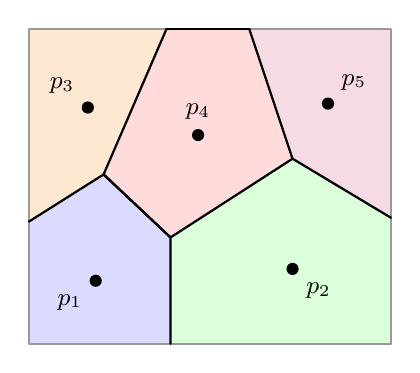
\begin{tikzpicture}[font=\small, line join=round, line cap=round, scale=1.0]
    \fill[blue!14] (0.2,0.2) -- (2.0,0.2) -- (2.0,1.55) -- (1.15,2.35) -- (0.2,1.75) -- cycle;
    \fill[green!14] (2.0,0.2) -- (4.8,0.2) -- (4.8,1.8) -- (3.55,2.55) -- (2.0,1.55) -- cycle;
    \fill[orange!18] (0.2,1.75) -- (1.15,2.35) -- (1.95,4.2) -- (0.2,4.2) -- cycle;
    \fill[red!14] (1.15,2.35) -- (2.0,1.55) -- (3.55,2.55) -- (3.0,4.2) -- (1.95,4.2) -- cycle;
    \fill[purple!14] (3.55,2.55) -- (4.8,1.8) -- (4.8,4.2) -- (3.0,4.2) -- cycle;

    \draw[thick, gray!80] (0.2,0.2) rectangle (4.8,4.2);
    \draw[thick] (2.0,0.2) -- (2.0,1.55) -- (1.15,2.35) -- (0.2,1.75);
    \draw[thick] (2.0,1.55) -- (3.55,2.55);
    \draw[thick] (1.15,2.35) -- (1.95,4.2);
    \draw[thick] (1.15,2.35) -- (2.0,1.55);
    \draw[thick] (3.55,2.55) -- (3.0,4.2);
    \draw[thick] (3.55,2.55) -- (4.8,1.8);
    \draw[thick] (1.95,4.2) -- (3.0,4.2);

    \foreach \x/\y/\name/\pos in {
        1.05/1.0/$p_1$/below left,
        3.55/1.15/$p_2$/below right,
        0.95/3.2/$p_3$/above left,
        2.35/2.85/$p_4$/above,
        4.0/3.25/$p_5$/above right}
    {
        \fill (\x,\y) circle (2.2pt);
        \node[\pos=2pt] at (\x,\y) {\name};
    }
\end{tikzpicture}
\caption{A Voronoi diagram in $\mathbb{R}^2$ for five sample sites. Each shaded cell contains the points closest to its generating site.}
\label{fig:voronoi-example}
\end{figure}

It will be important to note that Voronoi diagrams can be defined in any number of dimensions, however, we will be specifically interested in Voronoi diagrams in $\mathbb{R}^3$ for the purpose of this project.

There are several algorithms for computing these diagrams directly, including Fortune's algorithm and its beach-line sweep, however this type of algorithm does not easily generalize to higher dimensions. One option for computing Voronoi diagrams in higher dimensions is to use a divide and conquer approach (CITE Divide and conquer paper), however, the most common approach is to compute the Delaunay triangulation of the given point set and then extract the Voronoi diagram from the Delaunay triangulation \cite{delaunay_to_voronoi}. The Delaunay triangulation is a triangulation of a set of points that satisfies the Delaunay condition, which enforces that no point in the set can exist inside the circumcircle/sphere of any triangle/tetrahedron in the triangulation. A convenient property of Delaunay triangulations is that they are the dual of Voronoi diagrams, a property that is generalizable to any number of dimensions \cite{delaunay_to_voronoi}. An example of a Delaunay triangulation in $\mathbb{R}^2$ is shown in Figure~\ref{fig:delaunay-example}, where the points $p_i$ are shown as black dots, and the Delaunay triangulation is shown as a network of edges connecting the points. Note that this Delaunay triangulation is the dual of the Voronoi diagram shown in Figure~\ref{fig:voronoi-example}.

\begin{figure}[H]
\centering
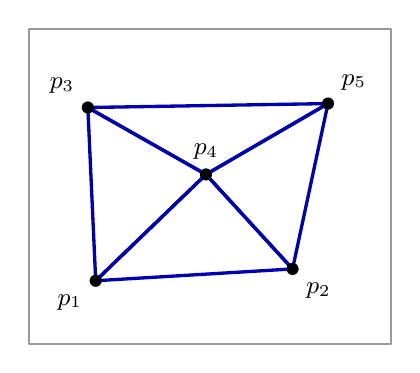
\begin{tikzpicture}[font=\small, line join=round, line cap=round, scale=1.0]
    \draw[thick, gray!80] (0.2,0.2) rectangle (4.8,4.2);

    \coordinate (p1) at (1.05,1.0);
    \coordinate (p2) at (3.55,1.15);
    \coordinate (p3) at (0.95,3.2);
    \coordinate (p4) at (2.45,2.35);
    \coordinate (p5) at (4.0,3.25);

    \draw[very thick, blue!70!black] (p1) -- (p2) -- (p4) -- cycle;
    \draw[very thick, blue!70!black] (p1) -- (p3) -- (p4) -- cycle;
    \draw[very thick, blue!70!black] (p2) -- (p5) -- (p4) -- cycle;
    \draw[very thick, blue!70!black] (p3) -- (p5) -- (p4) -- cycle;

    \foreach \x/\y/\name/\pos in {
        1.05/1.0/$p_1$/below left,
        3.55/1.15/$p_2$/below right,
        0.95/3.2/$p_3$/above left,
        2.45/2.35/$p_4$/above,
        4.0/3.25/$p_5$/above right}
    {
        \fill (\x,\y) circle (2.2pt);
        \node[\pos=2pt] at (\x,\y) {\name};
    }
\end{tikzpicture}
\caption{The Delaunay triangulation dual to Figure~\ref{fig:voronoi-example}. Two sites are connected when their Voronoi cells share an edge.}
\label{fig:delaunay-example}
\end{figure}

Since extracting the dual from a triangualtion is straightforward relative to the construction of the triangulation itself, we can compare the complexity of computing the Voronoi diagram to the complexity of computing the Delaunay triangulation, in which they are similar.

\subsection{Phonons}
Phonons are quasi-particles that represent quantized vibrational modes in a crystal lattice. This is to say that they are a way to describe the collective vibrations of atoms in a solid as if they were particles. You can think of phonons as quantum mechanical versions of classical sound waves, and as sound waves can be visualized as waves in a given medium, phonons can be visualized as wave/particles traveling through a crystal lattice. It is crucial to be able to study phonons in order to understand various properties of materials and is very important in the field of condensed matter physics.

\subsection{Reciprocal Lattices and Brillouin Zones}
A crystal lattice is a periodic arrangement of atoms in $\mathbb{R}^3$, which can be described by a set of basis vectors. A given lattice $L$ can be represented then as:

\begin{equation}
L = \{ n_1 a_1 + n_2 a_2 + n_3 a_3 | n_i \in \mathbb{Z} \}
\end{equation}

where $a_i$ are the basis vectors of the lattice.

A reciprocal lattice is a mathematical construct used in the study of periodic structures, crystal lattices being prime examples. It is derrived from the real-space lattice and is used to analyze wave phenomena in crystals. To get the reciprocal lattice, you can take the Fourier transform of the real-space lattice, which alludes to why this lattice lives in momentum space. It is important to note that the reciprocal lattice for a periodic structure is also periodic, exhibiting translational symmetry (i.e. shifting the lattice by by a reciprocal lattice vector leaves the lattice unchanged). We can represent the reciprocal lattice $L^*$ as:
\begin{equation}
L^* = \{ m_1 b_1 + m_2 b_2 + m_3 b_3 | m_i \in \mathbb{Z} \}
\end{equation}

where $b_i$ are the basis vectors of the reciprocal lattice, which can be calculated from the basis vectors of the real-space lattice, where:

\begin{equation}
b_i \cdot  a_j = 2\pi \delta_{ij}
\end{equation}

which means that the basis vectors of the reciprocal lattice are orthogonal to the basis vectors of the real-space lattice unless $i = j$, in which case they are parallel and have a magnitude of $2\pi$.

The First Brillouin zone (often just called the Brillouin Zone) is a fundamental region of k-space defined as the Wigner-Seitz cell of the reciprocal lattice, which gemetrically is represented as the Voronoi cell of the origin in the reciprocal lattice (where the lattice vector $G$ is zero). Due to the aforementioned periodicity (and subsequent translational symmetry) of the reciprocal lattice, the Brillouin zone contains all the unique wavevectors that can describe phonon propagation in the crystal lattice (all allowed values of $k$). The Brillouin zone is important for understanding the behavior of phonons in a crystal lattice, such as their dispersion relations and subsequently their group velocities, which are crucial for understanding thermal and electrical properties of materials.

\section{Computing Voronoi Diagrams in $\mathbb{R}^3$}
There are two algorithms we will discuss for computing Voronoi diagrams, which reduces to the method of computing the Delaunay triangulation in $\mathbb{R}^3$ of the given point set $P \in \mathbb{R}^3$ (the reciprocal lattice points). The first of which is the incremental construction algorithm for Delaunay Triangulations, a more intuitive approach, and the second of which is the lifting approach, which involves lifting the points in $\mathbb{R}^3$ to $\mathbb{R}^4$ and then computing the convex hull of the lifted points. For the three-dimensional setting and the extraction of the dual structure, our discussion follows the perspective described by Ledoux \cite{delaunay_to_voronoi}.

\subsection{Predicates}
\subsubsection{Orientation Test}
The orientation test is a fundamental predicate used in widely in computational gemoetry algorithms, including those for computing Delaunay triangulations \cite{lecture-notes-mount,lecture_notes_professor}. The purpose of an orientation test is to determine the relative orientation of a set of points in space. In $\mathbb{R}^3$, the orientation test for four points $a, b, c, d$ can be defined as follows:
\begin{equation}
    \textsc{Orient}(a, b, c, d) = \text{sign} \begin{vmatrix}
    a_x & a_y & a_z & 1 \\
    b_x & b_y & b_z & 1 \\
    c_x & c_y & c_z & 1 \\
    d_x & d_y & d_z & 1
    \end{vmatrix}
\end{equation}

In short, the orientation test computes the determinant of a matrix formed by the coordinates of the four points, and the determinant's sign indicates the relative orientation of the points. Our primary use of this orientation test will be to determine whether a point lies above, below, or on a plane defined by the three other points.

\subsubsection{In-Sphere Test}
The in-sphere test is another fundamental predicate used in computational geometry algorithms, and is constructed in a similar way to the orientation test. The in-sphere test for five points $a, b, c, d, e$ in $\mathbb{R}^3$ can be defined as follows:
\begin{equation}
    \textsc{InSphere}(a, b, c, d, e) = \text{sign} \begin{vmatrix}
    a_x & a_y & a_z & a_x^2 + a_y^2 + a_z^2 & 1 \\
    b_x & b_y & b_z & b_x^2 + b_y^2 + b_z^2 & 1 \\
    c_x & c_y & c_z & c_x^2 + c_y^2 + c_z^2 & 1 \\
    d_x & d_y & d_z & d_x^2 + d_y^2 + d_z^2 & 1 \\
    e_x & e_y & e_z & e_x^2 + e_y^2 + e_z^2 & 1
    \end{vmatrix}
\end{equation}

The reason why this test contains 5 points is because a sphere in $\mathbb{R}^3$ is defined by 4 points, and the in-sphere test determines whether the fifth point $e$ lies inside, outside, or on the sphere defined by the first four points $a, b, c, d$. The in-sphere test is crucial for maintaining the Delaunay condition during the construction of the Delaunay triangulation.

\subsection{Half-Faces and their Alignment}
In order to reliably use our defined predicates (orientation test/in sphere test), we must have a consistent ordering for vertices in faces. The order of vertices determines the result of the two tests (i.e. the way we construct the matrix) and thus we have to decide on a consistent convention. There are two ways that we will ensure this. The first, is to utilize the concept of "half-faces", which is the 3 dimentional version of a "half-edge". When we store the triangulation, we store each tetrahedron. Any tetrahedron can be constructed with 4 vertices, which we use to generate each half-face of the tetrahedron. Each half-face of the tetrahedron points outward, which can be ensured by performing an orientation test on the face to be constructed and the last remaining point in the Tetrahedron, and flipping vertices in the ordering until it returns $<0$. Each half-face can be the pair to another half-face, which represents two tetrahedra being adjacent along that face. In this case, both half-faces store a pointer to its pair. This enables both the efficient traversal between tetrahedra, and also the quick reconstructing of new tetrahedra during flipping, as faces can be reused from old tetrahedra that already point to relevant adjacent tetrahedra through its adjacent half-face.  

\subsection{Incremental Construction Algorithm for Delaunay Triangulations}
The incremental construction algorithm for Delaunay triangulations involves the insertion of points one at a time into an existing triangulation, and then updating the triangulation to maintain the global Delaunay property. Maintaining the Delaunay property involves a process called edge flipping, which is a local operation that replaces one edge of a triangulation with another edge to restore the Delaunay property. For the purpose of analysis, we will use randomized incremental construction, which involves inserting the points in a random order. 

To describe the algorithm, we will first define a few different functions that we will use in the algorithm. The first is a function that identifies the tetrahedron in the current triangulation that contains a given point $p$. The second is a function that checks whether a given tetrahedron violates the Delaunay condition, and the third is a function that 

To begin, we define the function \textsc{FindContainingTetrahedron} (Algorithm \ref{alg:find_containing_tetrahedron}) that takes in a Delaunay triangulation and a point, locating the tetrahedron in the triangulation that contains the point. This is done by starting with an arbitrary tetrahedron and then traversing the triangulation until we find the correct tetrahedron. This style of walk-based point location is closely related to the approach analyzed by M\"ucke, Saias, and Zhu \cite{muckeFastRandomizedPoint}.

Then we define the function \textsc{UpdateDelaunay} (Algorithm \ref{alg:insert_point_delaunay}) that takes in a Delaunay triangulation and a new point to be inserted, and updates the triangulation to include the new point while maintaining the Delaunay property. This utilizes our previously defined function \textsc{FindContainingTetrahedron} to find the tetrahedron that contains the new point, and then performs edge flips as necessary to restore the Delaunay property.

Finally, we can describe the overall Delaunay construction procedure itself. This routine begins with a super tetrahedron containing all input points, inserts the points one by one using Algorithm \ref{alg:insert_point_delaunay}, and then removes any tetrahedra incident to the vertices of the super tetrahedron.

\subsection{Computing Voronoi Diagrams from Delaunay Triangulations}
As mentioned previously, the Voronoi diagram of a set of points can be computed from the Delaunay triangulation of those points. This is because the dual of a Delaunay triangulation is the Voronoi diagram on the same set of points $P$. We want to extract 4 important pieces of information from the Delaunay triangulation in order to construct the Voronoi diagram: the vertices, edges, faces, and polyhedra (the cells) of the Voronoi diagram. We can extract the vertices of the Voronoi diagram from the circumcenters of the tetrahedra in the Delaunay triangulation, the edges of the Voronoi diagram from the shared faces of adjacent tetrahedra, the faces of the Voronoi diagram from the edges of the Delaunay triangulation, and the cells of the Voronoi diagram from the vertices of the Delaunay triangulation \cite{delaunay_to_voronoi}.



\subsection{Data Structures for Representing Delaunay Triangulations and Voronoi Diagrams}
It is important to note that the construction of a Voronoi diagram is not necessarily required in full. Rather, we can explicitly construct the Delaunay triangulation and simply query the necessary information from the triangulation using operations similar to those described in Algorithm \ref{alg:delaunay_to_voronoi} for targeted queries. For example, if we only want a single polygon in the Voronoi diagram, we can simply query the Delaunay triangulation for the necessary information to construct that single polygon without having to construct the entire Voronoi diagram. This idea will motivate why we will utilize a data structure most relevant for representing the Delaunay triangulation, as opposed to the Voronoi diagram. We will however store entire Voronoi diagrams for visualization purposes, but these need not be fast to construct, as they will not be used for querying.

Since the triangulation is in $\mathbb{R}^3$, we cannot use a DCEL (Doubly Connected Edge List) to represent the triangulation, as it is only suitable for representing planar subdivisions. Instead, we will store all tetrahedra in the triangulation, and for each tetrahedron, we will store pointers to its four vertices, its four faces, and its four adjacent tetrahedra. This way, we can easily navigate the triangulation and extract the necessary information for computing the First Brillouin zone as the Voronoi cell of the origin in the reciprocal lattice.

\subsection{Taking the Dual of a Delaunay Triangulation}
To take the dual of a Delaunay triangulation, we take advantage of the method described by \cite{delaunay_to_voronoi}, which describes how to extract the vertices, edges, faces, and cells of the Voronoi diagram from the Delaunay triangulation.

Let T be the DT of a set S of points in R3. The simplices of the dual D of T can be computed as follows (all the examples refer to Figure~\ref{fig:dual-examples}:

Vertex: a single Voronoi vertex is easily extracted:it is located at the centre of the sphere passing through the four vertices of its dual tetrahedron $\tau$.

Edge: a Voronoi edge, which is dual to a triangular face $\kappa$, is formed by the two Voronoi vertices dual to the two tetrahedra sharing $\kappa$.

Face: a Voronoi face, which is dual to a Delaunay edge, is formed by all the vertices that are dual to the Delaunay tetrahedra incident to $\alpha$. The idea is simply to 'turn' around a Delaunay edge and extract all the Voronoi vertices. These are guaranteed to be coplanar, and the face is guaranteed to be convex.

Polyhedron: the construction of one Voronoi cell Vp dual to a vertex p is similar: it is formed by all the Voronoi vertices dual to the tetrahedra incident to p. Since a Voronoi cell is convex by definition, it is possible to collect all the Voronoi vertices and then compute the convex hull (e.g. see [3] for an algorithm); the retrieval of all the tetrahedra incident to p can be done by performing a BFS-like algorithm on the graph dual to the tetrahedra. A simpler method consists of first identifying all the edges incident to p, and then extracting the dual face of each edge.
\begin{figure}[H]
    \centering
    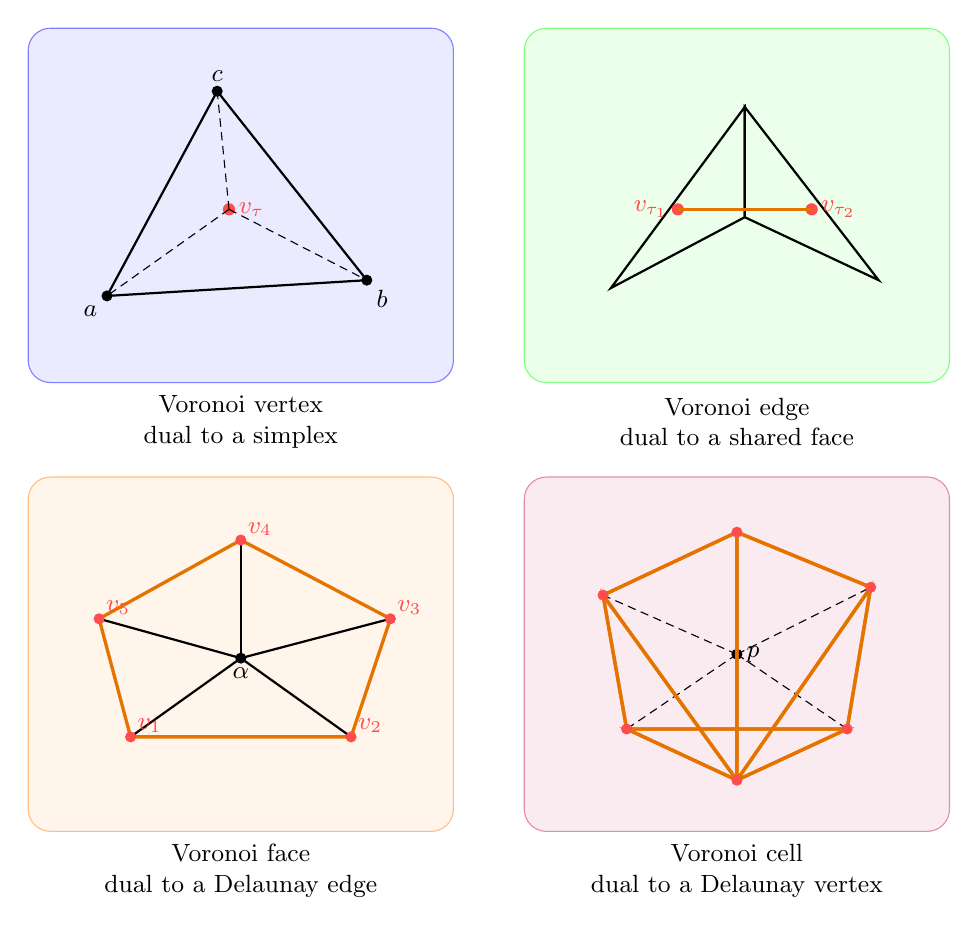
\begin{tikzpicture}[>=Latex, font=\small]
        \begin{scope}[xshift=0cm, yshift=0cm]
            \draw[rounded corners=8pt, fill=blue!8, draw=blue!50] (-0.2,-0.3) rectangle (5.2,4.2);
            \coordinate (a) at (0.8,0.8);
            \coordinate (b) at (4.1,1.0);
            \coordinate (c) at (2.2,3.4);
            \coordinate (o) at (2.35,1.9);
            \draw[thick] (a) -- (b) -- (c) -- cycle;
            \fill (a) circle (2pt) node[below left] {$a$};
            \fill (b) circle (2pt) node[below right] {$b$};
            \fill (c) circle (2pt) node[above] {$c$};
            \fill[red!70] (o) circle (2.2pt) node[right] {$v_\tau$};
            \draw[densely dashed] (o) -- (a);
            \draw[densely dashed] (o) -- (b);
            \draw[densely dashed] (o) -- (c);
            \node[align=center] at (2.5,-0.8) {Voronoi vertex \\ dual to a simplex};
        \end{scope}
    
        \begin{scope}[xshift=6.3cm, yshift=0cm]
            \draw[rounded corners=8pt, fill=green!8, draw=green!50] (-0.2,-0.3) rectangle (5.2,4.2);
            \coordinate (a1) at (0.9,0.9);
            \coordinate (b1) at (2.6,3.2);
            \coordinate (c1) at (4.3,1.0);
            \coordinate (d1) at (2.6,1.8);
            \draw[thick] (a1) -- (b1) -- (d1) -- cycle;
            \draw[thick] (c1) -- (b1) -- (d1) -- cycle;
            \fill[red!70] (1.75,1.9) circle (2.2pt) node[left] {$v_{\tau_1}$};
            \fill[red!70] (3.45,1.9) circle (2.2pt) node[right] {$v_{\tau_2}$};
            \draw[very thick, orange!90!black] (1.75,1.9) -- (3.45,1.9);
            \node[align=center] at (2.5,-0.8) {Voronoi edge \\ dual to a shared face};
        \end{scope}
    
        \begin{scope}[xshift=0cm, yshift=-5.7cm]
            \draw[rounded corners=8pt, fill=orange!8, draw=orange!50] (-0.2,-0.3) rectangle (5.2,4.2);
            \coordinate (e1) at (2.5,1.9);
            \coordinate (u1) at (1.1,0.9);
            \coordinate (u2) at (3.9,0.9);
            \coordinate (u3) at (4.4,2.4);
            \coordinate (u4) at (2.5,3.4);
            \coordinate (u5) at (0.7,2.4);
            \fill (e1) circle (2pt) node[below] {$\alpha$};
            \foreach \u in {u1,u2,u3,u4,u5}{
                \draw[thick] (e1) -- (\u);
            }
            \draw[very thick, orange!90!black] (u1) -- (u2) -- (u3) -- (u4) -- (u5) -- cycle;
            \foreach \u/\name in {u1/$v_1$,u2/$v_2$,u3/$v_3$,u4/$v_4$,u5/$v_5$}{
                \fill[red!70] (\u) circle (2pt) node[above right=-2pt and -1pt] {\name};
            }
            \node[align=center] at (2.5,-0.8) {Voronoi face \\ dual to a Delaunay edge};
        \end{scope}
    
        \begin{scope}[xshift=6.3cm, yshift=-5.7cm]
            \draw[rounded corners=8pt, fill=purple!8, draw=purple!45] (-0.2,-0.3) rectangle (5.2,4.2);
            \coordinate (s) at (2.5,1.95);
            \coordinate (w1) at (1.1,1.0);
            \coordinate (w2) at (3.9,1.0);
            \coordinate (w3) at (4.2,2.8);
            \coordinate (w4) at (2.5,3.5);
            \coordinate (w5) at (0.8,2.7);
            \coordinate (w6) at (2.5,0.35);
            \fill (s) circle (2pt) node[right] {$p$};
            \draw[densely dashed] (s) -- (w1);
            \draw[densely dashed] (s) -- (w2);
            \draw[densely dashed] (s) -- (w3);
            \draw[densely dashed] (s) -- (w4);
            \draw[densely dashed] (s) -- (w5);
            \draw[densely dashed] (s) -- (w6);
            \draw[very thick, orange!90!black] (w1) -- (w2) -- (w3) -- (w4) -- (w5) -- cycle;
            \draw[very thick, orange!90!black] (w1) -- (w2) -- (w6) -- cycle;
            \draw[very thick, orange!90!black] (w2) -- (w3) -- (w6) -- cycle;
            \draw[very thick, orange!90!black] (w3) -- (w4) -- (w6) -- cycle;
            \draw[very thick, orange!90!black] (w4) -- (w5) -- (w6) -- cycle;
            \draw[very thick, orange!90!black] (w5) -- (w1) -- (w6) -- cycle;
            \foreach \w in {w1,w2,w3,w4,w5,w6}{
                \fill[red!70] (\w) circle (2pt);
            }
            \node[align=center] at (2.5,-0.8) {Voronoi cell \\ dual to a Delaunay vertex};
        \end{scope}
    \end{tikzpicture}
    \caption{Duality between Delaunay simplices and Voronoi simplices. A Delaunay simplex gives a Voronoi vertex, a shared Delaunay face gives a Voronoi edge, a Delaunay edge gives a Voronoi face, and a Delaunay vertex gives an entire Voronoi cell.}
    \label{fig:dual-examples}
\end{figure}


\subsection{Setting up the Reciprocal Lattice and Computing the Brillouin Zone}

The details of how to set up the reciprocal lattice will depend on the specific crystal lattice we are working with, but the algorithm for computing the reciprocal lattice from a given real-space lattice is detailed in Algorithm \ref{alg:reciprocal_lattice}. This implementation handles any Bravais lattice, as we are working with the most ideal case.

There are a few important details to note about this algorithm. Since, for most of the implementation, we have been ensuring adhere to general position assumtptions. However, it is obvious that symmetric structures contain main violations of general position assumptions, especially Bravais lattices, which contain many points that are both Co-Planar and Co-Spherical. This can cause issues for the construction of the triangulation. We remedy this by adding a small perturbation to the points in the lattice, which helps us solve both of these problems. The perturbation is small enough such that it does not change the structure of the Voronoi diagram, and thus does not change the shape of the Brillouin zone, but it is large enough to break any co-planar or co-spherical configurations of points in the lattice.

\section{Results}

Below are two examples of computing Delaunay triangulations and Voronoi diagrams for two different Bravais lattices, the simple cubic lattice and tetragonal body centered lattice. The first Bravais lattice is the simple cubic lattice, which has a unit cell defined by three orthogonal vectors of equal length. The second Bravais lattice is the tetragonal body centered lattice, which has a unit cell defined by two orthogonal vectors of equal length and a third vector that is orthogonal to the first two but has a different length. Visualizations of the Delaunay triangulations and Voronoi diagrams for these two lattices are shown in Figure~\ref{fig:results_cubic} and Figure~\ref{fig:results_tetragonal}, respectively. 

\begin{figure}[H]
    \centering
    \begin{subfigure}{0.45\textwidth}
        \centering
        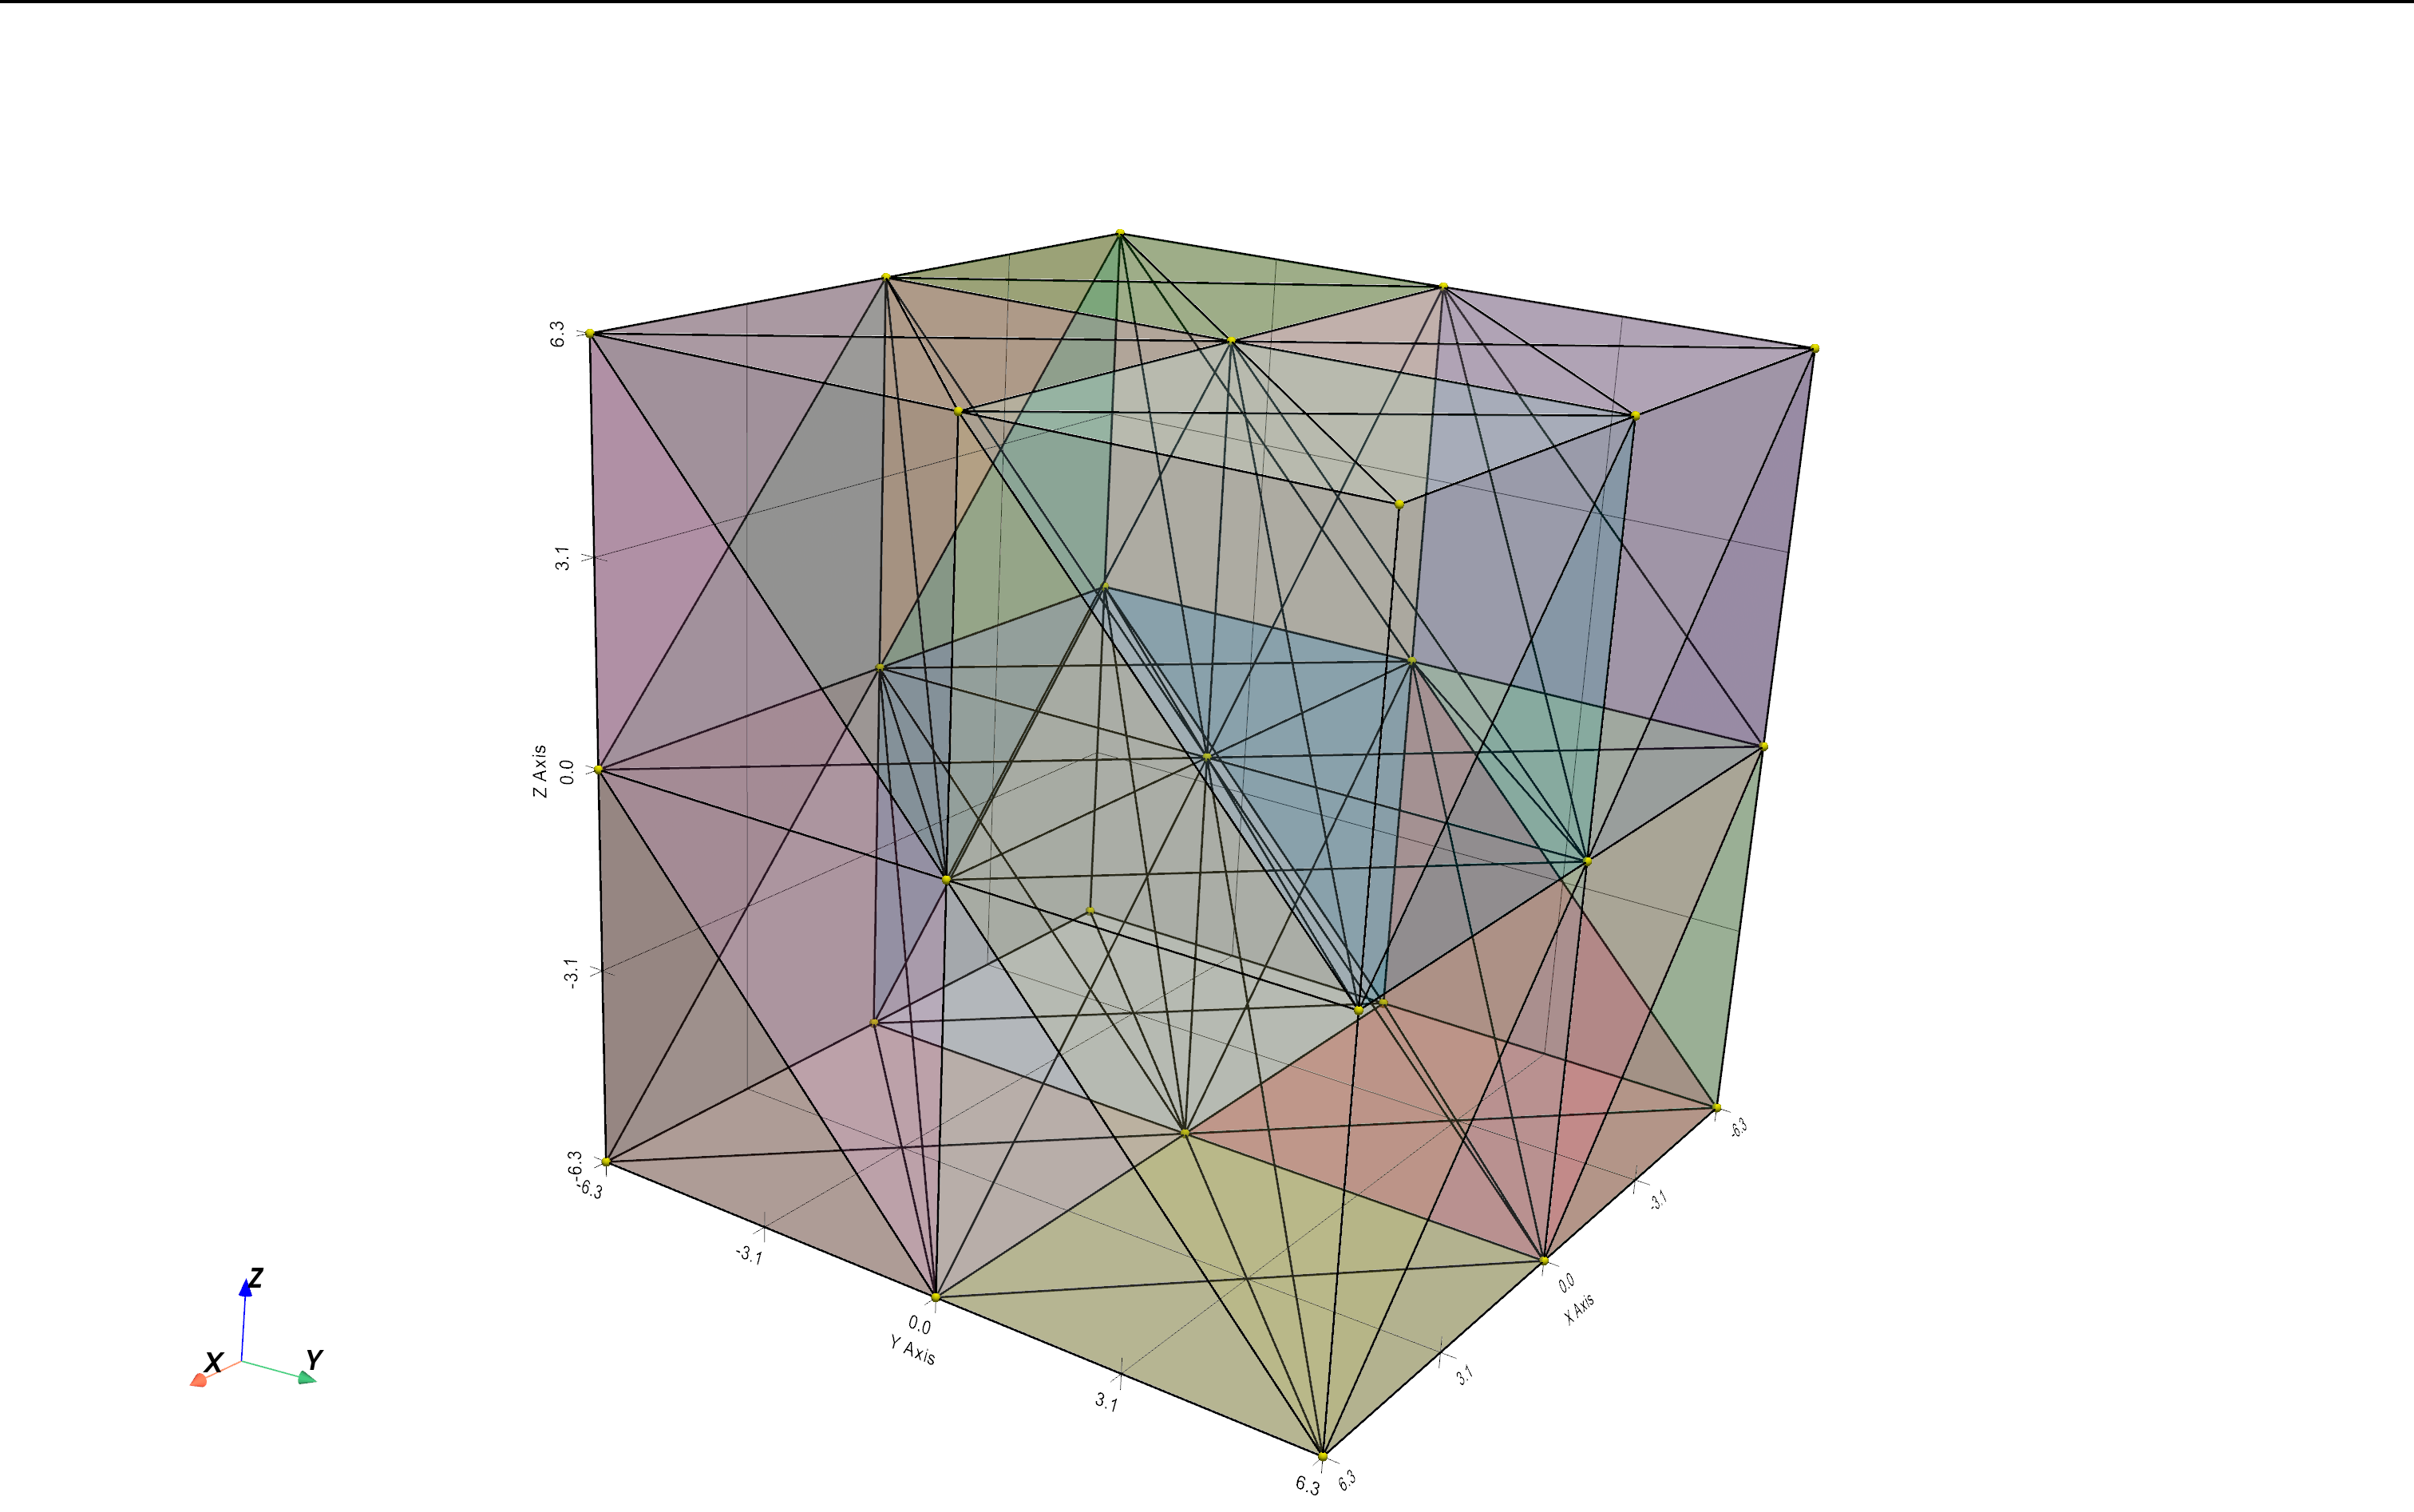
\includegraphics[width=\textwidth]{figures/triangulation_cubic.png}
        \caption{Delaunay triangulation of the reciprocal lattice of a simple cubic lattice.}
    \end{subfigure}
    \hfill
    \begin{subfigure}{0.45\textwidth}
        \centering
        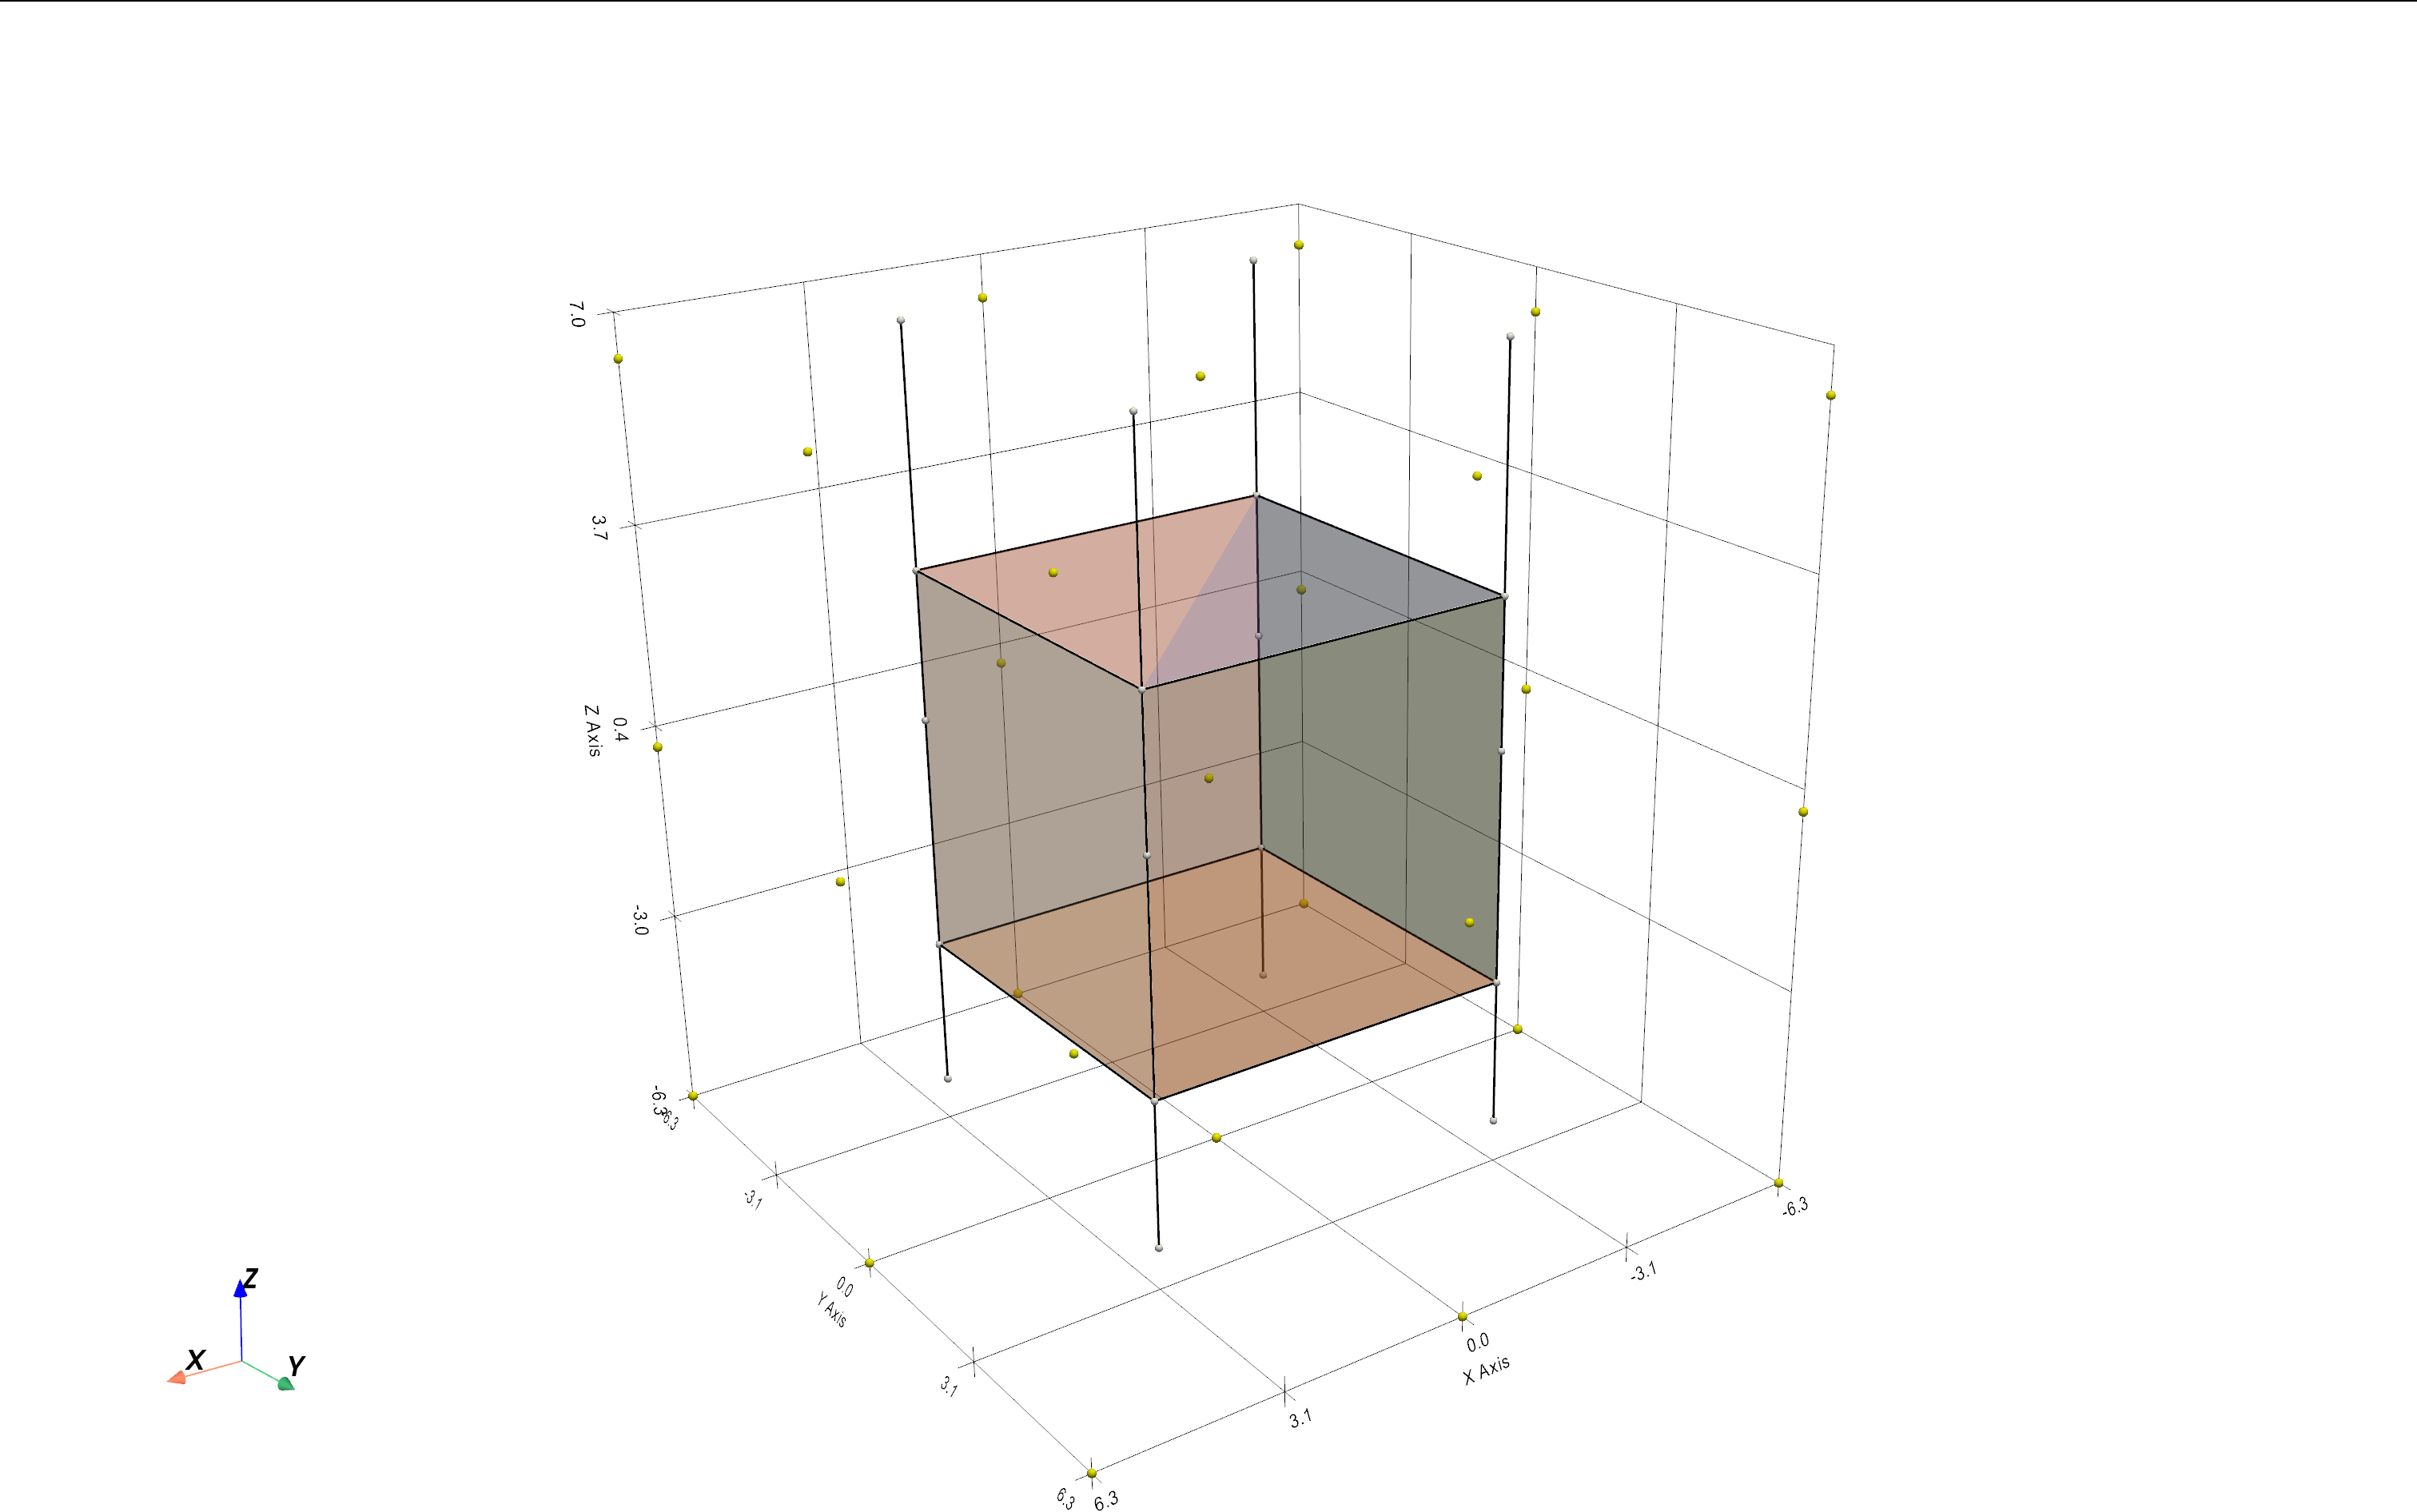
\includegraphics[width=\textwidth]{figures/voronoi_cubic.png}
        \caption{Voronoi diagram of the reciprocal lattice of a simple cubic lattice.}
    \end{subfigure}
    \caption{Delaunay triangulation and Voronoi diagram for the reciprocal lattice of a simple cubic lattice.}
    \label{fig:results_cubic}
\end{figure}

\begin{figure}[H]
    \centering
    \begin{subfigure}{0.45\textwidth}
        \centering
        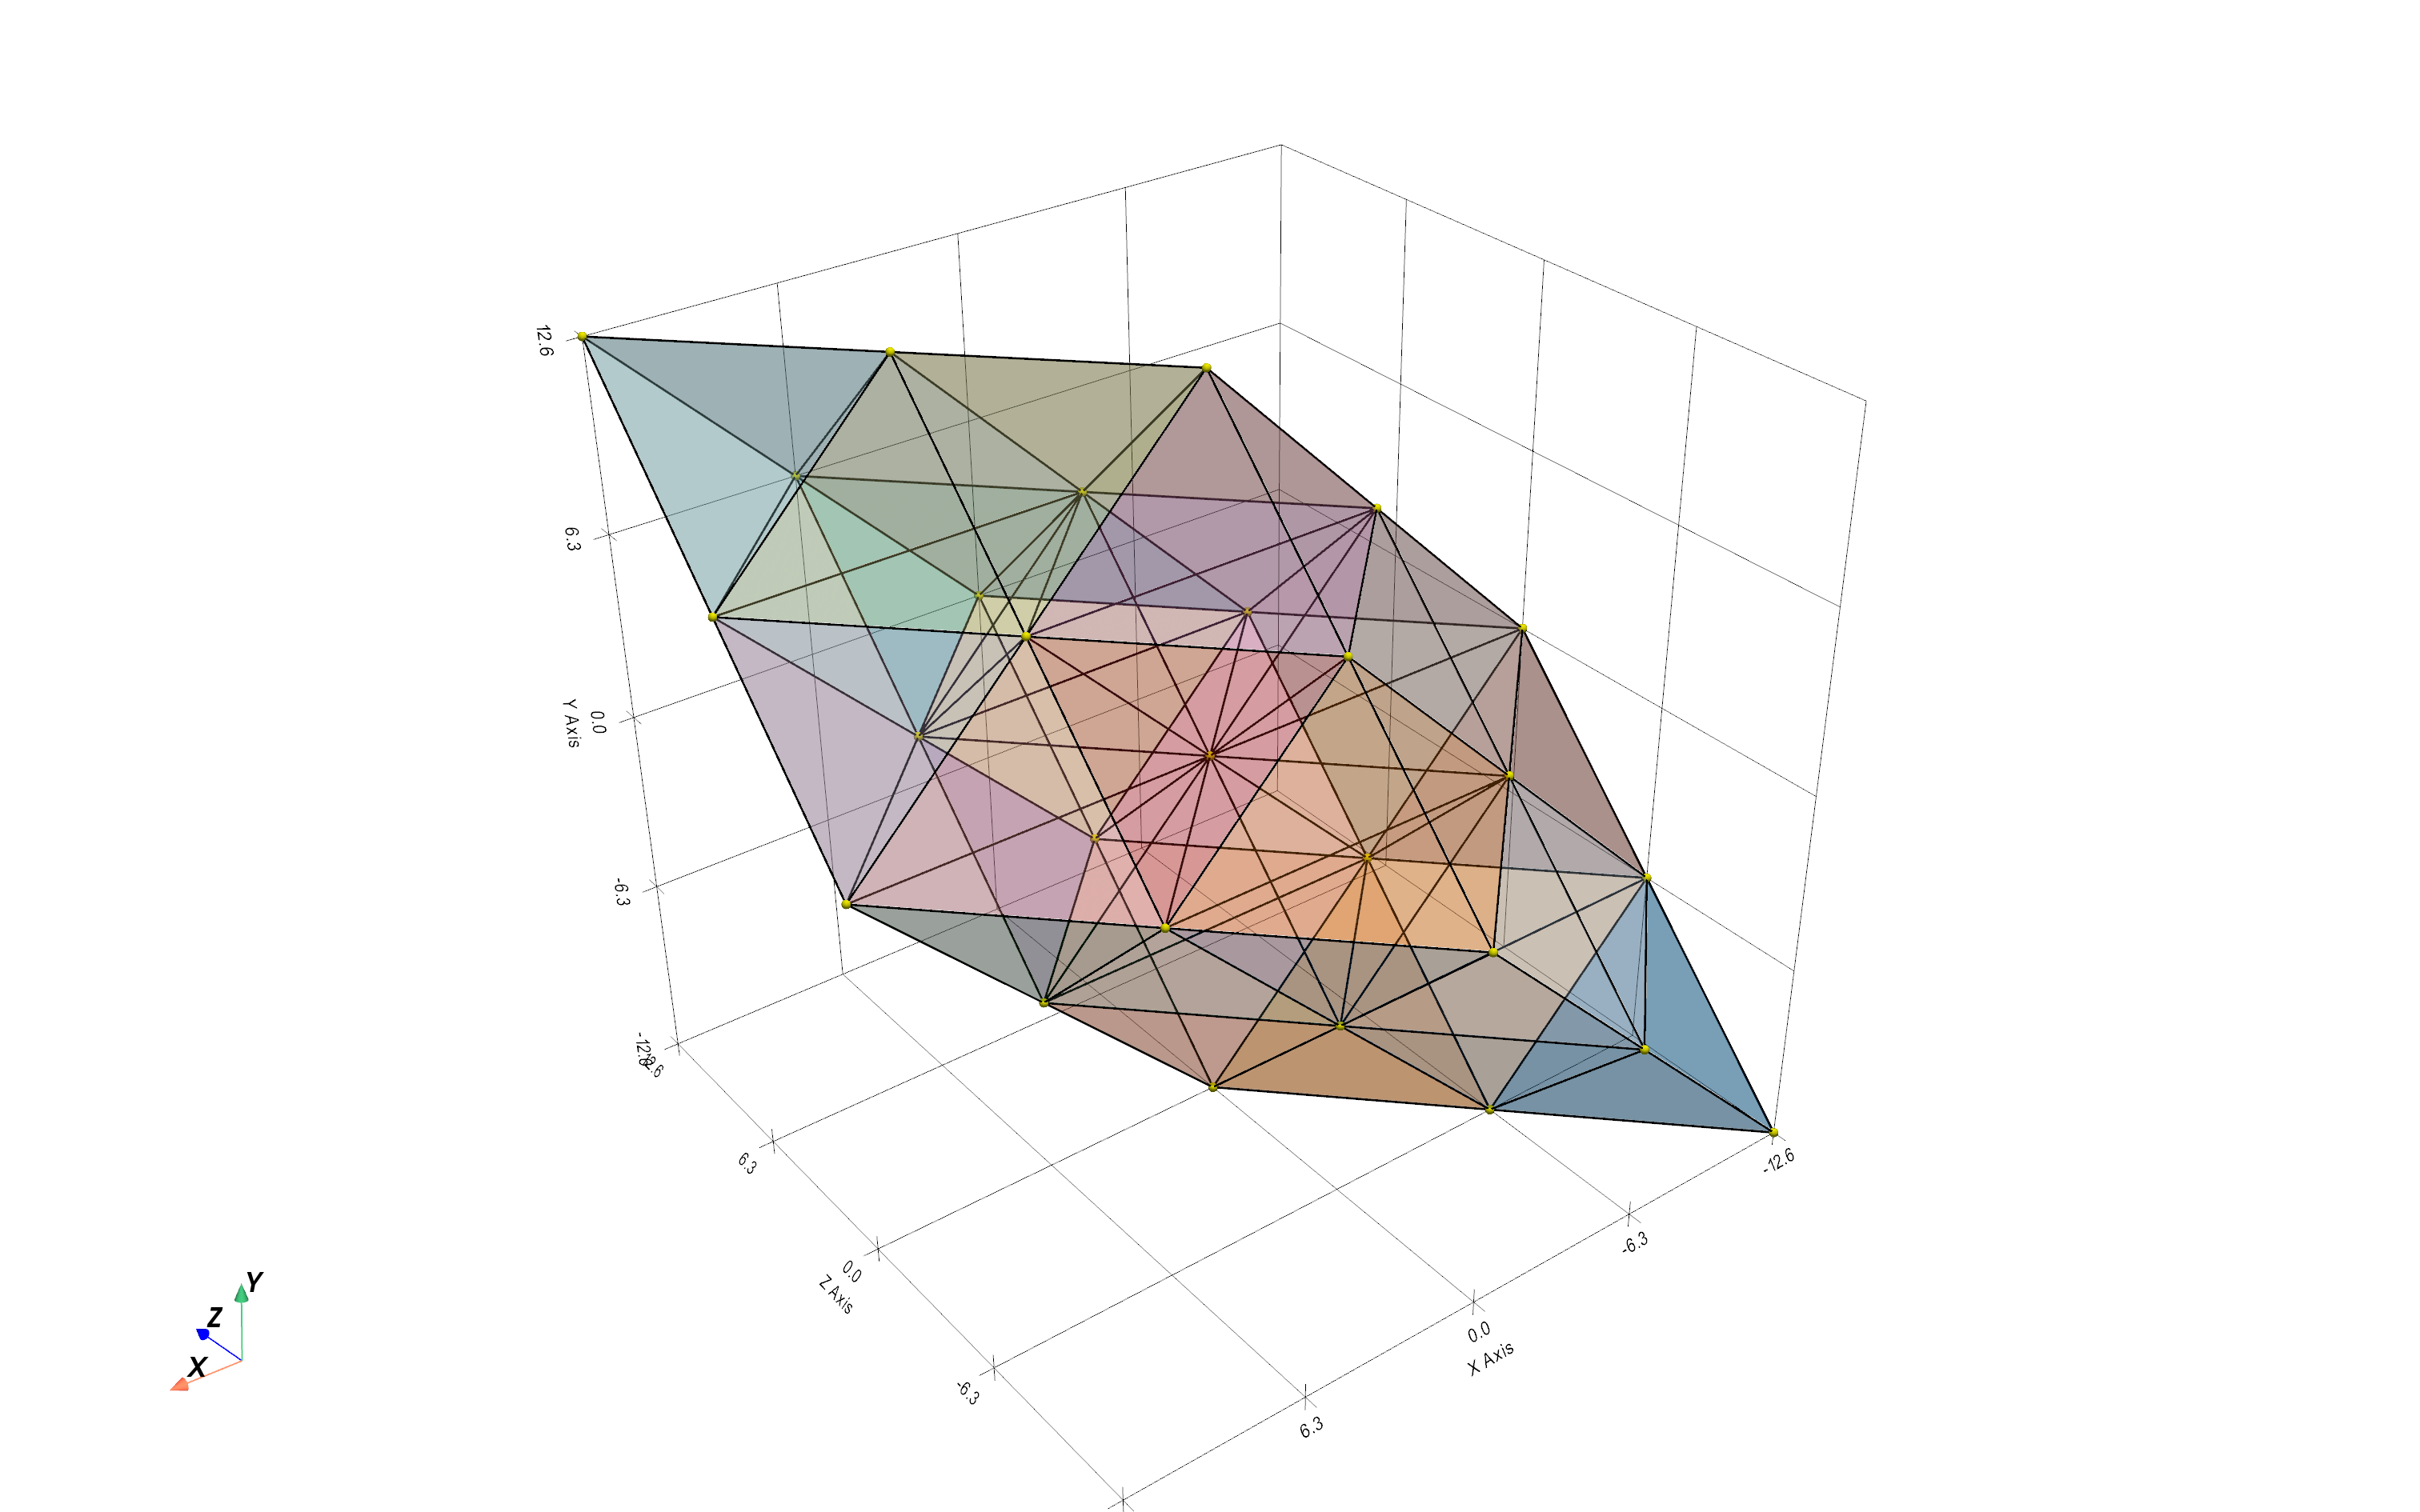
\includegraphics[width=\textwidth]{figures/triangulation_tetragonal.png}
        \caption{Delaunay triangulation of the reciprocal lattice of a tetragonal body centered lattice.}
    \end{subfigure}
    \hfill
    \begin{subfigure}{0.45\textwidth}
        \centering
        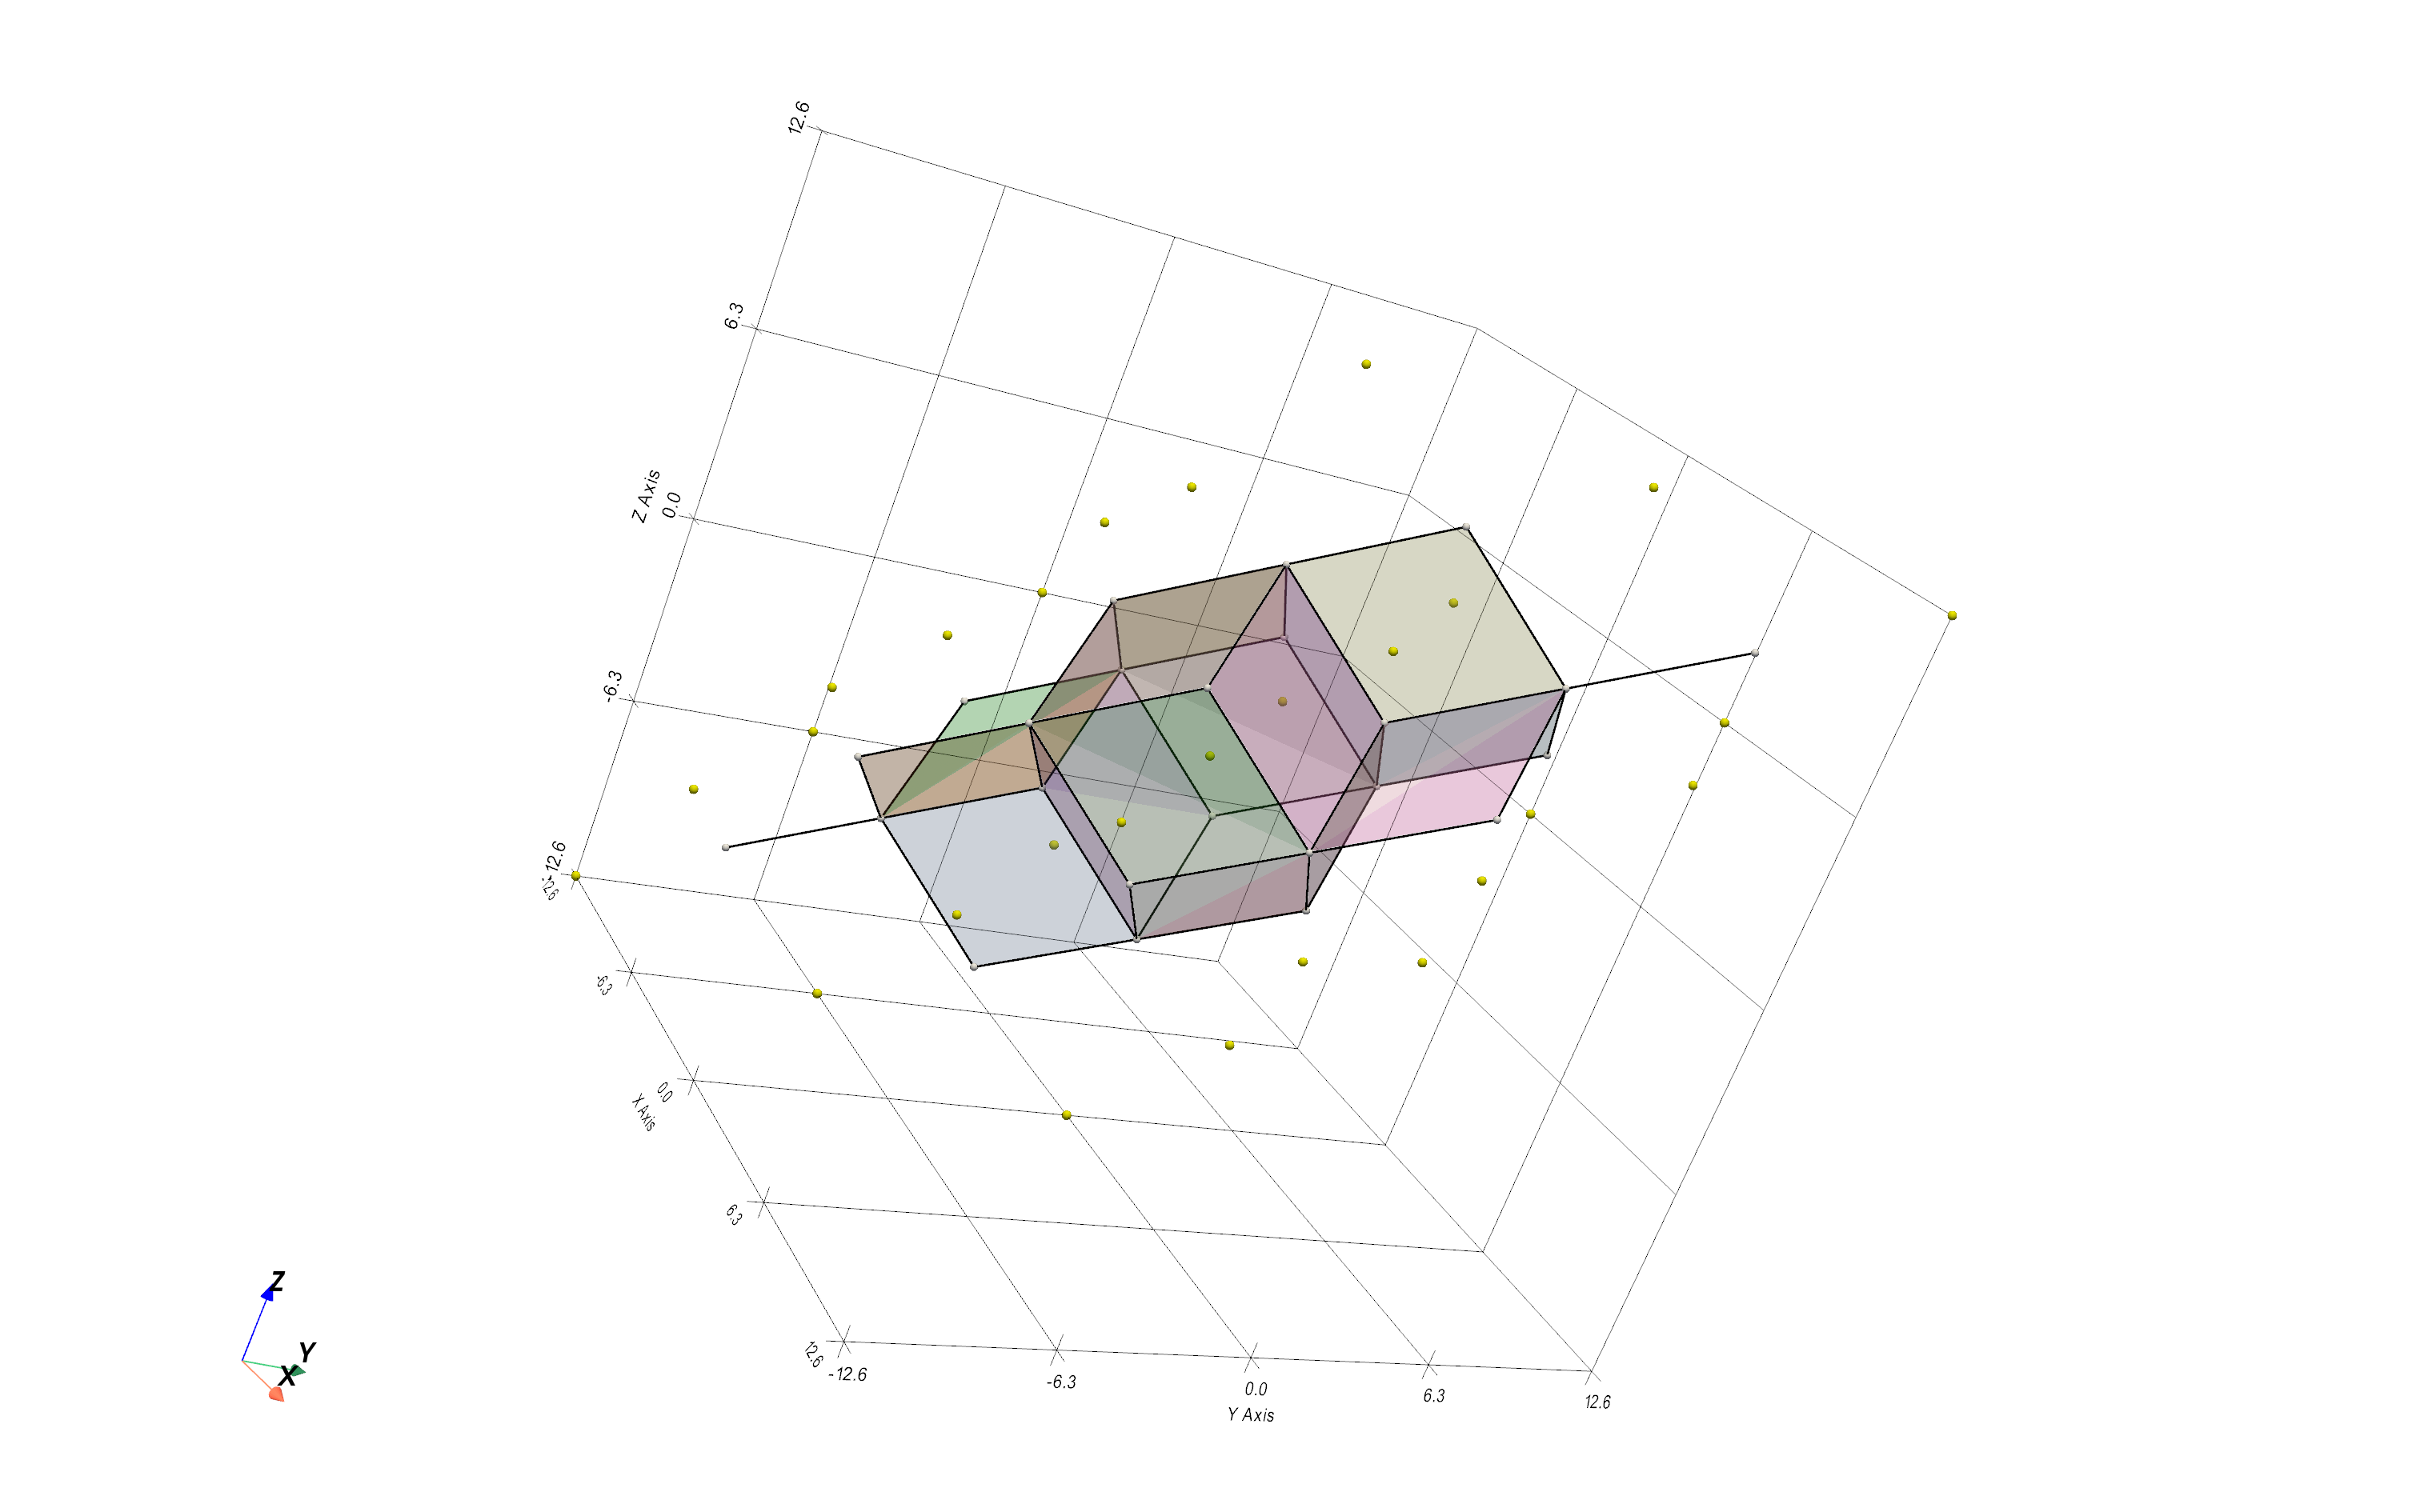
\includegraphics[width=\textwidth]{figures/voronoi_tetragonal.png}
        \caption{Voronoi diagram of the reciprocal lattice of a tetragonal body centered lattice.}
    \end{subfigure}
    \caption{Delaunay triangulation and Voronoi diagram for the reciprocal lattice of a tetragonal body centered lattice.}
    \label{fig:results_tetragonal}
\end{figure}

\section{Analysis}
The implementation can be split up into two main components: the construction of the Voronoi Diagram, and the construction of the reciprocal lattice. 

\subsection{Construction of the Voronoi Diagram}
The construction of the Voronoi diagram can also be split into two main components: the construction of the Delaunay triangulation, and the extraction of the Voronoi diagram from the Delaunay triangulation. The construction of the Delaunay triangulation's main bottleneck is the point location step, which walks through the triangulation to find the tetrahedron that contains the new point. While this, in the worst case, must walk through every tetrahedron and is thus $O(n)$, acording to \cite{muckeFastRandomizedPoint}, the expected complexity of this step is $O(n^{1/d})$, where $d$ is the dimension of the space, which in our case is 3. Thus making the expected complexity of the point location step $O(n^{1/3})$. The rest of the steps in the construction of the Delaunay triangulation are constant, but since this is an incremental construction algorithm, we have to perform this step for every point, which gives us an expected complexity of $O(n^{4/3})$ for the construction of the Delaunay triangulation. The extraction of the Voronoi diagram from the Delaunay triangulation is linear in the number of simplices in the triangulation, which is $O(n^2)$ in $\mathbb{R}^3$, thus giving us a complexity of $O(n^2)$ for this step. Thus, the overall expected complexity for the construction of the Voronoi diagram is $O(n^2)$.

\subsection{Construction of the Reciprocal Lattice}
The construction of the reciprocal lattice is linear in the number of points in the real-space lattice, which is $O(n)$, where $n$ is the number of points in the real-space lattice. This is because we can compute the basis vectors of the reciprocal lattice from the basis vectors of the real-space lattice in constant time, and then we can compute the points in the reciprocal lattice by taking integer linear combinations of the basis vectors, which is also linear in the number of points we want to compute. It may seem at first that there are 3 nested for loops, which would give us a complexity of $O(n^3)$, but these three nested for loops are iterating over each dimension of the lattice, and thus we only perform work for each point in the lattice, which gives us a complexity of $O(n)$.

\subsection{Overall Complexity}
It is clear that the bottleneck in our implementation is the construction of the Voronoi diagram, which has a complexity of $O(n^2)$, while the construction of the reciprocal lattice has a complexity of $O(n)$. Thus, the overall complexity of our implementation is $O(n^2)$.



\section{Future Work}
This project turned out to be significantly more difficult than we expected, so we did not get to implement every aspect outlined in our proposal. In particular, we were not able to simulate k-space trajectories through the Brillouin zone, which was the motivation behind the project. This is something we would like to implement in the future, as it would allow us to visualize the cyclic nature of the Brillouin zone and the advantage of symmetries in the study of crystal lattices and periodic structures in general. We would also like to implement a position-space visualization of the phonon modes in the crystal lattice, given my the k-sapce trajectories, but, this is a more ambitious goal that becomes more difficult as the k-space vector field becomes more complex. 


\nocite{lecture-notes-mount,lecture_notes_professor,chat-gpt}
\bibliographystyle{plain}
\bibliography{comp_geo}


\appendix
\section{Algorithms}


\begin{algorithm}
    \caption{Finding the Tetrahedron Containing a Point in a Delaunay Triangulation \\\hspace*{1em}\textbf{Input:} A Delaunay triangulation $T$ of a point set $P$ in $\mathbb{R}^3$, and a point $p$ to be located.\\\hspace*{1em}\textbf{Output:} The tetrahedron $t$ in $T$ that contains the point $p$.}
    \label{alg:find_containing_tetrahedron}
\begin{algorithmic}[1]
    \Procedure{FindContainingTetrahedron}{$T$, $p$}
        \Let $t$ be an arbitrary tetrahedron in $T$.
        \Let $V$ be the set of visited Tetrahedra
        \Let $out = None$
        \While{true}
            \If{$t \in V$}
                \State Return $None$
            \EndIf
            \State Add $t$ to $V$
            \For{each face $f_i$ of $t$}
                \If \textsc{Orient}($f_i$[0], $f_i$[1], $f_i$[2], $p$) $> \varepsilon$
                    \State Set $out$ to $f_i$
                    \State break
                \EndIf
            \EndFor
        \If{$out = None$}
            \State Return $t$
        \Else
            \If{the pair of $out$ does not exist}
                \State Return $None$
            \Else
                \State Let $t$ be the tetrahedron of the pair of $out$
                \State Set $out = None$
            \EndIf
        \EndIf
        \EndWhile
    \EndProcedure
\end{algorithmic}
\end{algorithm}

\begin{algorithm}
\caption{Insertion of a Point into a Delaunay Triangulation \\\hspace*{1em}\textbf{Input:} A current Delaunay triangulation $T$ of a point set $P$ in $\mathbb{R}^3$, and a new point $p$ to be inserted.\\\hspace*{1em}\textbf{Output:} An updated Delaunay triangulation $T'$ that includes the new point $p$.}
\label{alg:insert_point_delaunay}
\begin{algorithmic}[1]
    
    \Procedure{UpdateDelaunay}{$T$, $p$}
        \State Find the tetrahedron $t$ in $T$ that contains $p$.
        \State Subdivide $t$ into four new tetrahedra by connecting $p$ to the vertices of $t$.
        \State Reconnect the new tetrahedra to the adjacent tetrahedra of $t$.
        \State Connect pairs of new tetrahedra that share a face.
        \State Remove $t$ from $T$ and add the four new tetrahedra to $T$.
        \State Initialize a queue $Q$ with the new tetrahedra.
        \While{$Q$ is not empty}
            \State Dequeue a tetrahedron $t'$ from $Q$.
            \If{$t'$ is no longer in $T$}
                \State continue
            \EndIf
            \For{each face $f$ of $t'$}
                \If{the pair of $f$ exists}
                    \Let $t''$ be the tetrahedron of the pair of $f$
                    \Let $v$ be the vertex of $t''$ opposite to $f$
                    \If{$v$ lies strictly inside the circumsphere of $t'$}
                        \State Perform a local flip between $t'$ and $t''$.
                        \State Enqueue the new tetrahedra formed by the flip into $Q$.
                        \State break
                    \EndIf
                \EndIf
            \EndFor
        \EndWhile
        \State \textbf{return} the updated triangulation $T'$.
    \EndProcedure
\end{algorithmic}
\end{algorithm}

\begin{algorithm}
\caption{Constructing a Delaunay Triangulation \\\hspace*{1em}\textbf{Input:} A point set $P$ in $\mathbb{R}^3$.\\\hspace*{1em}\textbf{Output:} A Delaunay triangulation $T$ of $P$.}
\label{alg:construct_delaunay}
\begin{algorithmic}[1]
    \Procedure{ConstructDelaunay}{$P$}
        \State Construct a super tetrahedron $T_{large}$ containing all points of $P$.
        \State Initialize the triangulation $T$ to contain only $T_{large}$.
        \For{each point $p$ in $P$}
            \State Set $T \gets$ \textsc{UpdateDelaunay}($T$, $p$).
        \EndFor
        \State Initialize an empty list $T'$.
        \For{each tetrahedron $\tau$ in $T$}
            \If{$\tau$ contains no vertex of $T_{large}$}
                \State Add $\tau$ to $T'$.
            \EndIf
        \EndFor
        \State \textbf{return} $T'$.
    \EndProcedure
\end{algorithmic}
\end{algorithm}

\begin{algorithm}
\caption{Computing the Voronoi Diagram from a Delaunay Triangulation \\ \hspace*{1em}\textbf{Input:} A Delaunay triangulation $T$ of a point set $P$ in $\mathbb{R}^3$.\\\hspace*{1em}\textbf{Output:} The Voronoi diagram $V$ of the point set $P$.}
\label{alg:delaunay_to_voronoi}
\begin{algorithmic}[1]
    \Procedure{DelaunayToVoronoi}{$T$}
        \State Initialize an empty Voronoi diagram $V$.
        \State Initialize maps from tetrahedra to Voronoi vertices, from Delaunay edges to incident tetrahedra, and from Delaunay vertices to incident tetrahedra.
        \For{each tetrahedron $\tau$ in $T$}
            \State Compute the circumcenter of $\tau$ and add it as a vertex in $V$.
            \State Record the circumcenter associated with $\tau$.
            \State For each vertex of $\tau$, record that $\tau$ is incident to that vertex.
            \State For each edge of $\tau$, record that $\tau$ is incident to that edge.
        \EndFor
        \For{each tetrahedron $\tau$ in $T$}
            \For{each face $\kappa$ of $\tau$}
                \State Let $t'$ be the tetrahedron adjacent to $\tau$ across $\kappa$.
                \State If $t'$ exists, add an edge in $V$ between the circumcenters of $\tau$ and $t'$.
            \EndFor
        \EndFor
        \For{each edge $\alpha$ in $T$}
            \State Let $t_1, t_2, ..., t_k$ be the tetrahedra incident to $\alpha$.
            \State Order $t_1, t_2, ..., t_k$ by turning around $\alpha$ through adjacent faces.
            \State Let $v_1, v_2, ..., v_k$ be the circumcenters of $t_1, t_2, ..., t_k$.
            \State Add the finite chain $v_1, v_2, ..., v_k$ as the Voronoi face dual to $\alpha$.
            \State Add edges $(v_i, v_{i+1})$ for each consecutive pair.
            \State If the first and last tetrahedra are also adjacent around $\alpha$, add the closing edge $(v_k, v_1)$.
        \EndFor
        \For{each vertex $p$ in $T$}
            \State Let $t_1, t_2, ..., t_m$ be the tetrahedra incident to $p$.
            \State Identify all Delaunay edges incident to $p$.
            \State Collect the Voronoi faces dual to those edges.
            \State Add a cell in $V$ using the vertices contained in those faces.
        \EndFor
        \State \textbf{return} the Voronoi diagram $V$.
    \EndProcedure
\end{algorithmic}
\end{algorithm}

\begin{algorithm}
    \caption{Setting Up a Reciprocal Lattice \\\hspace*{1em}\textbf{Input:} A Bravais lattice type $L$, lattice parameters $a,b,c,\alpha,\beta,\gamma$, and an index range $r$.\\\hspace*{1em}\textbf{Output:} A finite reciprocal lattice point set $P$, together with direct basis vectors $a_1,a_2,a_3$ and reciprocal basis vectors $b_1,b_2,b_3$.}
    \label{alg:setup_reciprocal_lattice}
    \begin{algorithmic}[1]
        \Procedure{SetupReciprocalLattice}{$L, a,b,c,\alpha,\beta,\gamma,r$}
            \State Normalize the lattice type $L$ to one of the $14$ Bravais lattice types.
            \State Construct primitive direct basis vectors $a_1,a_2,a_3$ from the lattice type and parameters.
            \State Compute the cell volume $V = a_1 \cdot (a_2 \times a_3)$.
            \State Compute reciprocal basis vectors
            \State $b_1 = 2\pi \dfrac{a_2 \times a_3}{V}$, $b_2 = 2\pi \dfrac{a_3 \times a_1}{V}$, $b_3 = 2\pi \dfrac{a_1 \times a_2}{V}$.
            \State Initialize an empty point set $P$.
            \For{$i=-r$ to $r$}
                \For{$j=-r$ to $r$}
                    \For{$k=-r$ to $r$}
                        \State Let $p = i b_1 + j b_2 + k b_3$.
                        \State Add $p$ to $P$.
                    \EndFor
                \EndFor
            \EndFor
            \State Apply a small deterministic perturbation to the points of $P$.
            \State \textbf{return} $P, (a_1,a_2,a_3), (b_1,b_2,b_3)$.
        \EndProcedure
    \end{algorithmic}
    \end{algorithm}




\end{document}
